\chapter{Arquitetura proposta}

\section{Visão geral do sistema}


\begin{figure}[H]
  \centering
  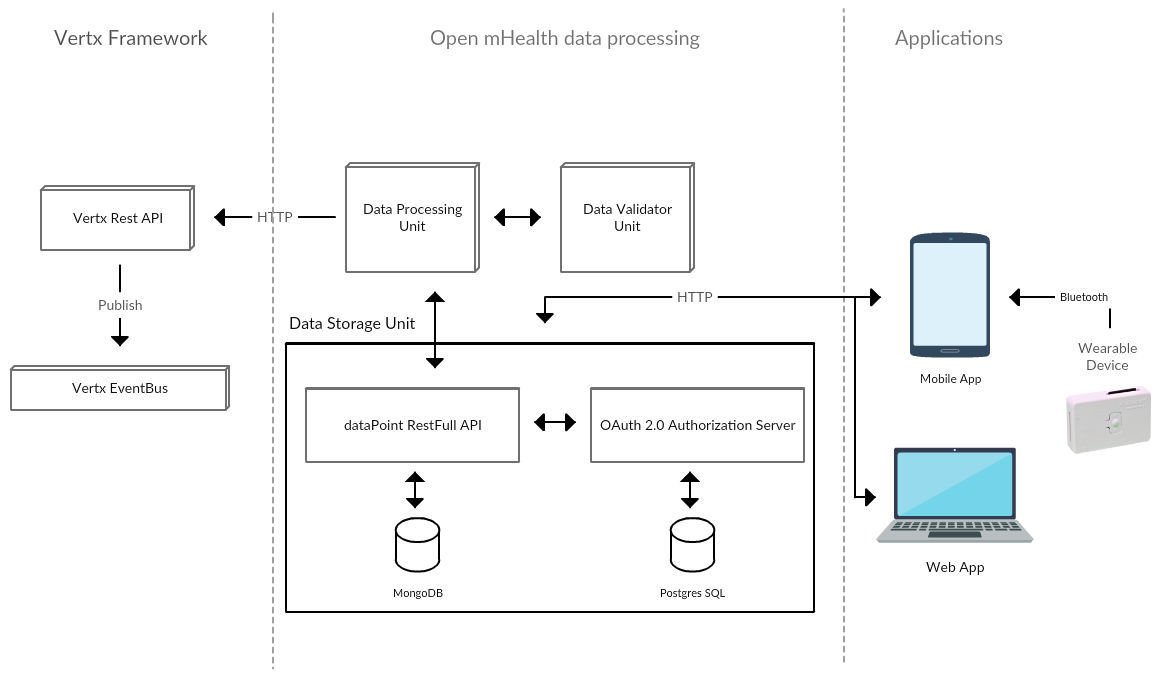
\includegraphics[width=1\textwidth]{imgs/arch-product.png}
  \caption[Arquitetura do Sistema]{Arquitetura do Sistema}
  
  \label{f:product-arch}
\end{figure}

%Apresentação da arquitetura do sistema global, com texto de suporte, para descrever como as partes se relacionam
A arquitetura proposta para o sistema estará dividida em três partes. Uma delas é a parte das aplicações desenvolvidas, ou seja, a interface com o utilizador, tanto web como móvel. Estas duas aplicações comunicarão por pedidos \gls{HTTP} com o \gls{DSU} da framework do Open mHealth. A aplicação móvel ainda terá a possibilidade de se ligar ao \gls{VJ} por bluetooth para receber os dados fisiológicos da pessoa que está a efetuar a colheita.
\par 
Uma outra parte do sistema já referida é o backend do Open mHealth. Este backend tem um componente principal (\gls{DSU}) que dispobilizará duas \gls{REST} \gls{API} para inserção e fornecimento dos dados e ainda para autenticação e autorização. Ainda terá um componente para processar os dados recebidos. Estes dados passarão por um validador. e podem ser reencaminhados para o Vert.x por pedidos \gls{HTTP}.
\par
A terceira e última parte é composta pelo Vert.x, é fornecida uma \gls{API} \gls{REST} que possibilitará a receção dos dados para posterior publicação dos mesmo no EventBus.
\section{Módulos do sistema}
% a ideia é apresentar de forma mais detalhada os componentes que foram ilustrados na secção anterior e qual é o plano técnico para a sua implementação. Notar que a idei é escrever um plano/especificação ANTES de haver a implementação. cada uma das secções (pus aqui algumas, podem ser outras) deve rfletir um dos módulos importantes da arquitetura
\subsection{Fundações do backend}
Composto por um servidor de autenticação e autorização utilizando spring(citar o spring) 
\subsection{API de integração}
\subsection{Gestão de utilizadores e acessos}
\subsection{Extensão com módulos personalizados}


\section{Modelo do domínio}

% descrever as estruturas de dados que vão ser usadas (o nosso Reference information model) 

\section{Proteção de dados}


%  como é que a arquitetura proposta contribui para a preservação de privacidade e segurança dos dados?

\cleardoublepage